\chapter{Результаты и их обсуждение}
\label{ch:results}

\section{Экспериментальная установка}
Для нахождения вязкости воздуха в тонкой трубке использовалась установка, изображённая на рис. 1. Поток воздуха под давлением, немного превышающим атмосферное, поступал через газовый счётчик в тонкие металлические трубки. Регулировалась интенсивность подачи воздуха. Для нахождения разности давлений на концах трубки использовался микроманометр, а для измерения давления газа на входе - водяной U-образный манометр.

\begin{figure}[h!]
        \centering
        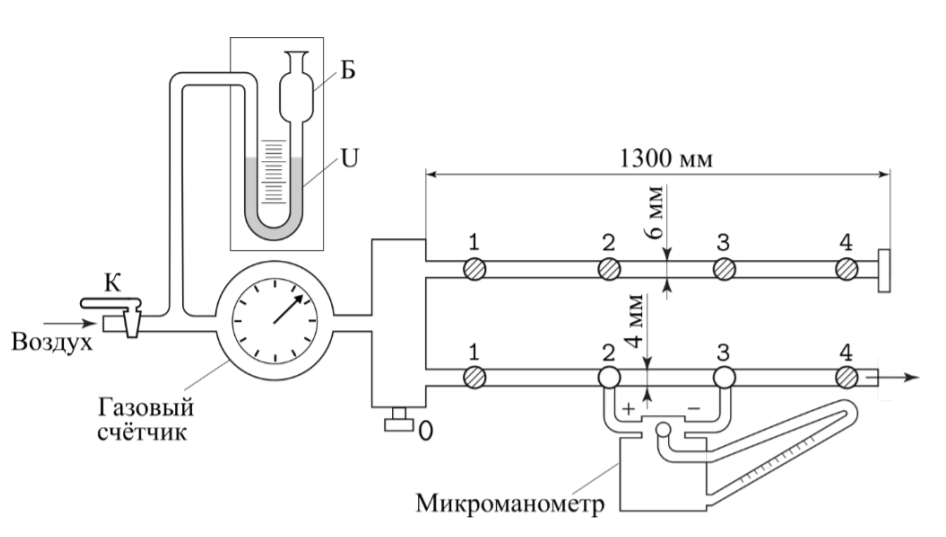
\includegraphics[scale=0.5]{img/expust.png}
        \caption{\centering Экспериментальная установка для нахождения коэффициента вязкости воздуха в тонкой трубке. Поток воздуха под давлением, немного превышающим атмосферное, поступал через газовый счётчик в тонкие металлические трубки. Регулировалась интенсивность подачи воздуха. Для нахождения разности давлений на концах трубки использовался микроманометр, а для измерения давления газа на входе - водяной U-образный манометр.}
\end{figure} 
Полное описание установки смотри в приложении А. 
    
\section{Обработка результатов измерений}

Чтобы использовать формулу Пуазейля для нахождения вязкости воздуха в тонкой трубке экспериментально нашли зависимости расхода от перепада давления для трёх трубок разного внутреннего диаметра (результаты измерений см. в Приложении Б.), построили по ним графики и нашли на них участки с линейной зависимости $Q (\Delta P)$(см. рис. 2 - 3).

\begin{figure}[ht]
\centering
    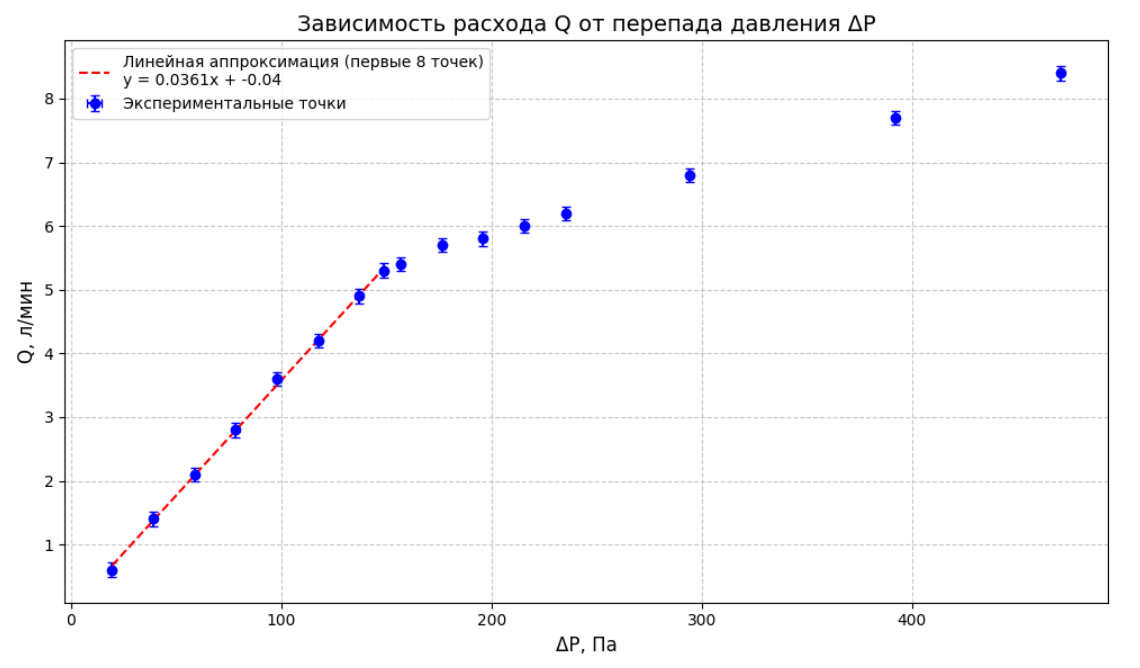
\includegraphics[width = \textwidth]{img/Q(dP)d=3,95.png}
    \begin{center}
    Рис. 2. График зависимости $Q (\Delta P)$ для трубки диаметром d = 3.95 мм. Синими точками на графике показаны экспериментальные данные. Через первые 8 точек проведена прямая, чтобы выделить участок с ламинарным течением. Коэффициент наклона линейного участка графика составил k = 0.0361. %(полностью описание) для чего, что на рисунке
    \end{center}
\end{figure}
\newpage

\begin{figure}[ht]
\centering
    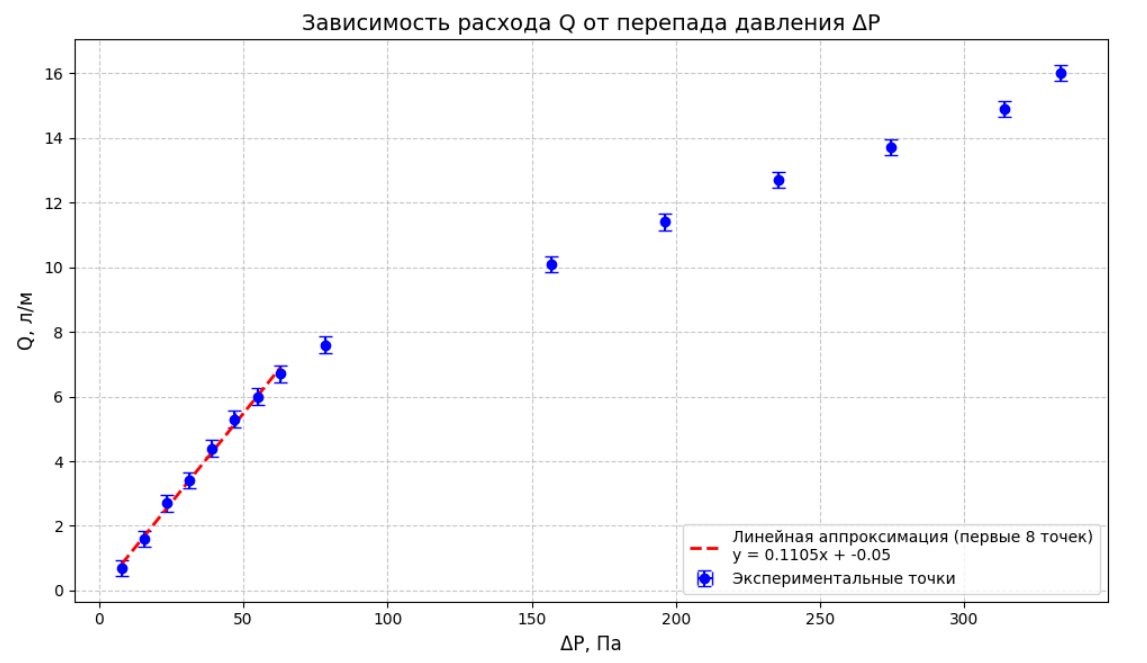
\includegraphics[width = \textwidth]{img/Q(dP)d=5,05.png}
    \begin{center}
    Рис. 3. График зависимости $Q (\Delta P)$ для трубки диаметром d = 5.05 мм.  Синими точками на графике показаны экспериментальные данные. Через первые 8 точек проведена прямая, чтобы выделить участок с ламинарным течением. Коэффициент наклона линейного участка графика составил k = 0.1105.  %(полностью описание) для чего, что на рисунке
    \end{center}
\end{figure}

Вязкость воздуха в каждой трубке нашли используя коэффициенты наклона линейных участков графиков из формулы Пуазейля (1). Значения в пределах погрешности совпали с табличным значением $\eta_{\text{табл}} =  1,832 \cdot 10^{-5} \, \text{Па}. \cdot \text{с}$ \cite{Lab}. Это показывает, что использование формулы Пуазейля позволяет оценить вязкость воздуха в тонкой трубке. %но и справедливы те посылки, для которых была построена теория и выведена формула Пуазейля
Для оценки длины установления в тонких трубках по формуле (2) рассчитали число Рейнольдса для условий первой и второй трубки (см. Табл. 1).

\begin{table}[h]
\centering
\begin{tabular}{|c|c|c|}
 \hline
{$d$, мм} & {$\eta$, $\cdot 10^{-5}$ Па/c} & Re \\
 \hline
3.95 & $2.0 \pm 0.2$ & $1560 \pm 160$\\ \hline
5.05 & $1.7 \pm 0.4$ & $1600 \pm 400$\\ \hline
\end{tabular}
\caption{
\centering Коэффициенты вязкости, полученные для каждой трубки из формулы Пуазейля с использованием коэффициента наклона линейной части графиков зависимости Q от $\Delta P$.
}
\end{table}

Построили графики по результатам измерений зависимостей отношения давления к длине трубки от координаты вдоль трубы $\Delta P/l(x)$ (см. рис 4, 5). Из графиков оценили длину участка, на котором происходит установление потока. Сравнили результат с оценкой по формуле (2)(см. Табл. 2). Полученные из графиков значения разошлись со значениями, полученными при оценке, менее чем на 15\%, это показывает, что метод оценки по формуле (2) позволяет с точностью до 15\% определить длину установления. Однако, из-за недостатка точек оказалось невозможно с достаточной точностью обнаружить по графику переход к установившемуся состоянию.

\begin{figure}[ht]
\centering
    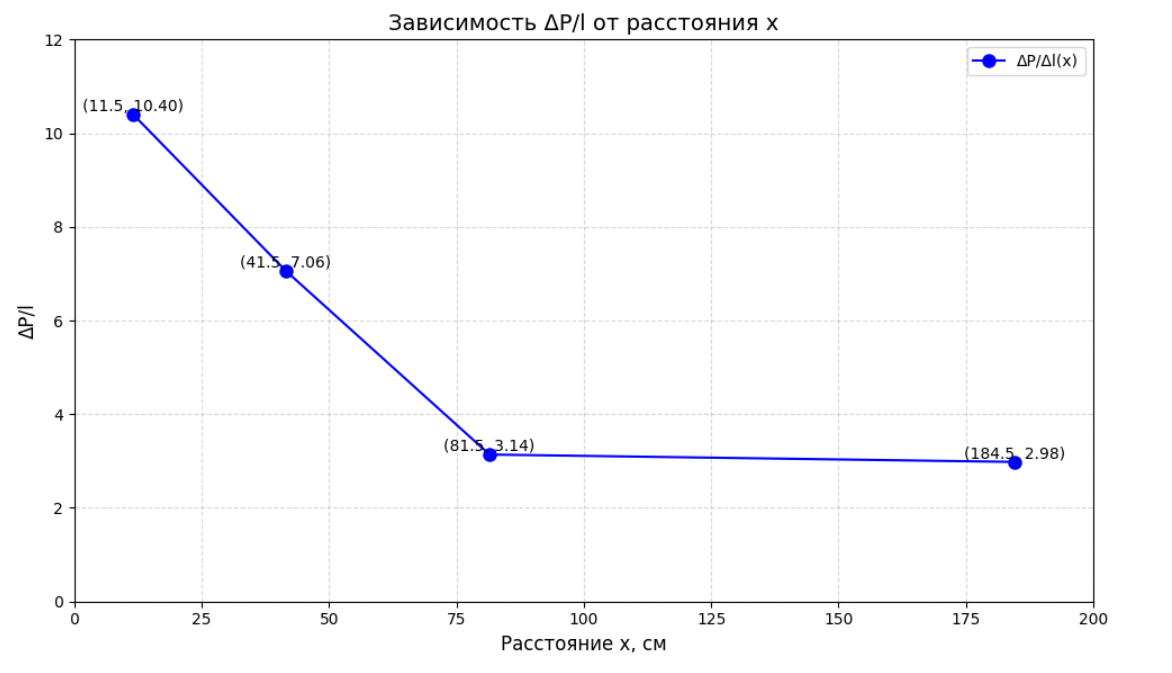
\includegraphics[width = \textwidth]{img/dPl(x)d=3,95.png}
    \begin{center}
    Рис. 4. График зависимости $\Delta P/l(x)$ для трубки диаметром $d = 3.95$. Синими точками на графике показаны полученные данные. Синие линии проведены между точками для удобства определения начала линейного участка.  %(полностью описание) для чего, что на рисунке
    \end{center}
\end{figure}
\newpage

\begin{figure}[ht]
\centering
    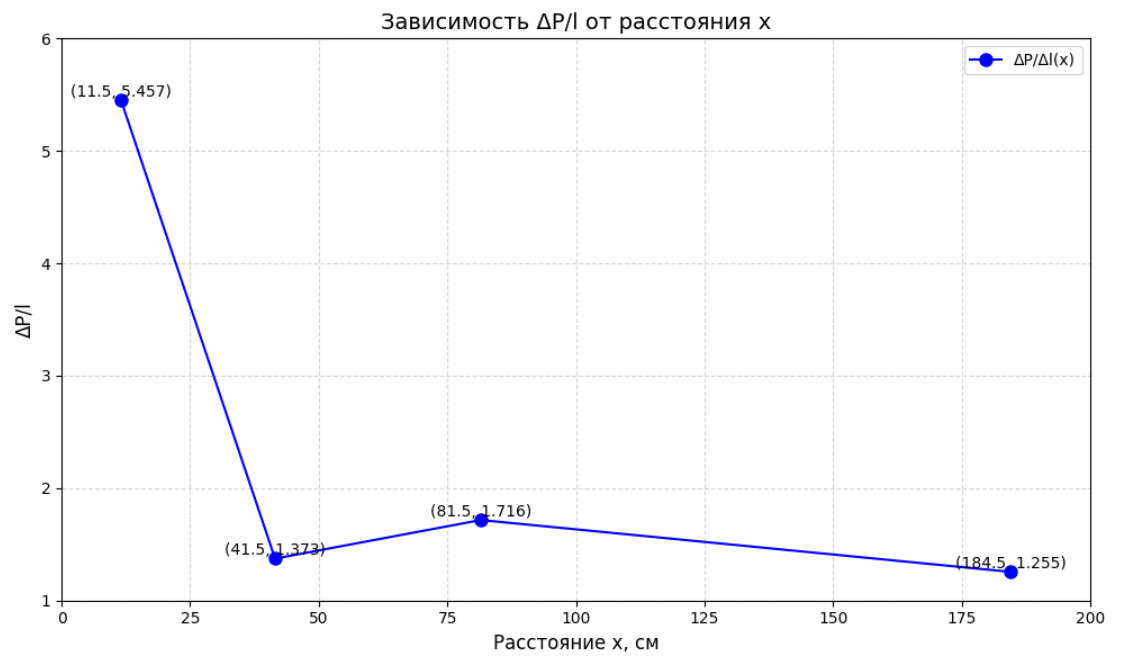
\includegraphics[width = \textwidth]{img/dPl(x)d=5,05.png}
    \begin{center}
    Рис. 5. График зависимости $\Delta P/l(x)$ для трубки диаметром $d = 5.05$. Синими точками на графике показаны полученные данные. Синие линии проведены между точками для удобства определения начала линейного участка. %(полностью описание) для чего, что на рисунке
    \end{center}
\end{figure}

\begin{table}[h]
\centering
\begin{tabular}{|c|c|c|}
 \hline
{$d$, мм} & {$l_\text{уст}$, см} & {$l_\textbf{уст}$ по формуле, см}\\
 \hline
3.95 & 70.0 & 62.4 \\ \hline
5.05 & 80.0 & 80.2 \\ \hline
\end{tabular}
\caption{
\centering Длины установления для каждой трубки, определённые по графику зависимости $\Delta P/l(x)$ и оценки длины установления по формуле (2).
}
\end{table}

Для сравнения с теоретической зависимостью расхода от радиуса трубки - коэффициента $\beta$ в отношении $Q \propto R^\beta$ для ламинарного и турбулентного течения, провели дополнительные измерения (см. Табл. 3). Получили, что коэффициент $\beta_\text{лам} = 1.7$ для ламинарного течения и $\beta_\text{турб} = 3.0$ для турбулентного течения. Значение для ламинарного и турбулентного течения не сошлось с теоретическими значениями $\beta_{\text{лам}_\text{теор}} = 4$,  $\beta_{\text{турб}_\text{теор}} = 2.5$. Это говорит о том, что теоретическая модель описания турбулентного течения и метод размерностей для ламинарного течения оказались неприменимы для данного эксперимента.

\begin{table}[h]
\centering
\label{tab:flow_regimes}
\begin{tabular}{|c|c|c|c|c|c|}
\hline
\multicolumn{3}{|c|}{\textbf{Ламинарный режим}} & \multicolumn{3}{c|}{\textbf{Турбулентный режим}} \\ \hline
$d$, мм & $\Delta P/\Delta l$, Па/см & $Q$, л/мин & $d$, мм & $\Delta P/\Delta l$, Па/см & $Q$, л/мин \\ \hline
3.95 & $0.980 \pm 0.019$ & $7.8 \pm 0.08$ & 3.95 & $5.88 \pm 0.05$ & $6.80 \pm 0.07$ \\ \hline
5.05 & $0.980 \pm 0.019$ & $11.80 \pm 0.12$ & 5.05 & $5.88 \pm 0.05$ & $14.20 \pm 0.14$ \\ \hline
\end{tabular}
\caption{\centering Данные для нахождения коэффициента $\beta$ в отношении $Q \propto R^\beta$ для ламинарного и турбулентного течения.}
\end{table}
